\documentclass{article}

\usepackage[preprint]{neurips_2026}
\usepackage[utf8]{inputenc}
\usepackage[T1]{fontenc}
\usepackage{microtype}
\usepackage{graphicx}
\usepackage{booktabs}
\usepackage{tabularx}
\usepackage{array}
\usepackage{amsmath,amssymb,mathtools}
\usepackage{xcolor}
\usepackage{enumitem}
\usepackage{multirow}
\usepackage{url}
\usepackage{pifont}

\definecolor{encblue}{HTML}{2676A8}
\definecolor{priororange}{HTML}{D56A32}
\definecolor{decgreen}{HTML}{27876A}
\definecolor{teacherpurple}{HTML}{7158A6}
\definecolor{cautionred}{HTML}{B7463B}
\definecolor{softgray}{HTML}{56616A}
\newcommand{\enc}[1]{\textcolor{encblue}{#1}}
\newcommand{\prior}[1]{\textcolor{priororange}{#1}}
\newcommand{\dec}[1]{\textcolor{decgreen}{#1}}
\newcommand{\teacher}[1]{\textcolor{teacherpurple}{#1}}
\newcommand{\caution}[1]{\textcolor{cautionred}{#1}}
\newcommand{\yes}{\textcolor{decgreen}{\ding{51}}}
\newcommand{\no}{\textcolor{cautionred}{\ding{55}}}
\newcommand{\stopgrad}{\operatorname{sg}}
\newcommand{\E}{\mathbb{E}}
\newcommand{\KL}{D_{\mathrm{KL}}}
\newcommand{\R}{\mathbb{R}}
\newcommand{\method}[1]{\textsc{#1}}

\title{Representations for Generation:\\
A Survey of the Convergence of Visual Representation Learning and Generative Modeling}

\author{%
  Kieran Didi\\
  NVIDIA\\
  \texttt{kieran.didi@gmail.com}
}

\begin{document}

\maketitle

\begin{abstract}
Visual generation was long organized around a modular bargain: learn a perceptual compressor, freeze it, and train a generative model in its latent space. Representation learning developed in parallel, optimizing invariances for recognition rather than invertibility or likelihood. Since 2024 these lines have converged through representation-aligned denoisers, semantically shaped tokenizers, representation autoencoders, jointly learned latent priors, and native self-supervised generators. The resulting literature is difficult to compare because terms such as \emph{representation}, \emph{latent}, \emph{end-to-end}, and \emph{unified} conceal different gradient paths. We organize the field by two axes: where a representation enters the system, and how strongly representation and generation are coupled. We derive the objectives behind representative methods, isolate six properties of a useful generative latent---fidelity, semantics, information rate, modelability, geometry, and decoder robustness---and distinguish exact mathematical claims from empirical design hypotheses. We then connect the visual literature to language, multimodal systems, and molecular or 3D structure generation. Our main conclusion is deliberately non-monolithic: no single representation is universally best. The correct interface depends on which information should survive compression, which errors occur at inference, and which components are allowed to shape one another. This is a curated survey with a literature cutoff of 7 September 2026.
\end{abstract}

\section{Introduction}

Modern generative systems increasingly contain two learners that are easy to conflate. A \emph{representation learner} maps data \(x\) to features \(z\) that expose useful factors of variation. A \emph{generator} learns a probability distribution over \(x\), or over a latent \(z\) from which \(x\) can be decoded. The former is usually rewarded for invariance; the latter ultimately pays for every visually consequential detail. Their objectives can cooperate, but they can also disagree.

Latent diffusion made this tension operational. A separately trained autoencoder first compresses images, and a diffusion or flow model then learns the latent distribution \citep{vahdat2021lsgm,rombach2022ldm}. This separation enabled efficient scaling, but it fixed the interface before the generator could express what it found easy or difficult. Meanwhile, self-supervised encoders such as DINO, DINOv2, MAE, and CLIP learned strong semantic features \citep{caron2021dino,oquab2023dinov2,he2022mae,radford2021clip}. The recent representations-for-generation literature asks what happens when these features supervise, initialize, replace, or co-evolve with the generative latent.

The literature is often narrated as a sequence: align denoiser features; align the autoencoder; discard the conventional VAE in favor of a foundation-model encoder; finally train representation and generation jointly. That chronology is useful, but not a taxonomy. \method{REPA-E}, \method{UNITE}, \method{Unified Latents} (UL), and \method{GenFirst} can all be called end-to-end while transmitting materially different gradients. \method{Self-Flow} learns internal features without an external vision foundation model (VFM), but does not thereby eliminate latent compression. \method{Latent Forcing} co-denoises semantic features and pixels, yet does not learn a tokenizer. A model can share parameters without allowing every objective to update every representation.

This survey makes four contributions:
\begin{enumerate}[leftmargin=*,nosep]
  \item a two-axis taxonomy based on \emph{intervention point} and \emph{training coupling};
  \item a common mathematical language for auxiliary alignment, pretrained-feature latents, rate-controlled joint latent learning, and native self-supervision;
  \item an evaluation framework that separates six latent properties and explicitly traces gradient flow; and
  \item cross-domain case studies showing what changes in language, unified multimodal models, and molecular or 3D structure generation.
\end{enumerate}

\paragraph{Scope and evidence.}
We focus on diffusion, flow-matching, and autoregressive systems for which learned representations are a primary design variable. This is a curated technical survey, not a systematic review or a leaderboard. Many 2026 results are preprints with incomparable compute, guidance, sampling, and evaluation protocols. We label a company announcement as product evidence rather than as a reproducible method, and use social-media posts only for discovery and context. Unless otherwise stated, numerical claims belong to the cited paper's own protocol.

\paragraph{Central thesis.}
The choice of latent is a constrained interface-design problem. A useful code must preserve what the decoder cannot cheaply hallucinate while presenting a distribution that the prior can learn. Reconstruction and recognition probe only parts of that contract. Information rate, covariance and spectral structure, manifold geometry, exposure to off-manifold inputs, and the exact gradient path can dominate.

\section{A Common Mathematical Language}
\label{sec:math}

\subsection{The modular latent generator}

Let data \(x\sim p_{\mathrm{data}}\), encoder \(q_\phi(z\mid x)\), decoder \(p_\psi(x\mid z)\), and learned prior \(p_\theta(z)\). A modular latent generator performs
\[
 x \xrightarrow{\;\enc{q_\phi}\;} z
 \qquad\text{and}\qquad
 z_0\sim p_\theta \xrightarrow{\;\dec{p_\psi}\;} \hat{x}.
\]
The interface \(z\) serves two clients with different wishes. The decoder prefers a code rich enough for faithful reconstruction. The prior prefers a regular, low-complexity distribution. A semantic learner may prefer invariance to texture, pose, or instance detail. Latent quality therefore cannot be a single scalar.

For a variational autoencoder (VAE), introduce an auxiliary posterior \(q_\phi(z\mid x)\). The marginal log likelihood obeys
\begin{align}
\log p_{\theta,\psi}(x)
&= \log \int q_\phi(z\mid x)
  \frac{p_\theta(z)p_\psi(x\mid z)}{q_\phi(z\mid x)}\,dz \nonumber\\
&\ge
\underbrace{\E_{q_\phi(z\mid x)}[\log p_\psi(x\mid z)]}_{\dec{\text{reconstruction}}}
-
\underbrace{\KL(q_\phi(z\mid x)\|p_\theta(z))}_{\prior{\text{rate / prior match}}}
\equiv \mathcal{L}_{\mathrm{ELBO}}(x),
\label{eq:elbo}
\end{align}
where the inequality is Jensen's. The color code will be used throughout: \enc{blue} denotes encoder or representation terms, \prior{orange} denotes prior or generative terms, \dec{green} denotes decoder terms, and \teacher{purple} denotes external or target representations.

Equation~\eqref{eq:elbo} exposes the classic trade-off but hides two practical facts. First, perceptual and adversarial reconstruction losses need not correspond to a normalized likelihood. Second, a simple analytic prior such as \(\mathcal{N}(0,I)\) can be replaced by a learned diffusion prior. The resulting system can be trained jointly, in stages, or with selected stop-gradients. These choices change the optimization problem even when the forward graph looks identical.

\subsection{Diffusion and flow objectives}

In a variance-preserving diffusion parameterization \citep{ho2020ddpm,song2021sde},
\begin{equation}
 z_t = \alpha_t z_0+\sigma_t\epsilon,\qquad
 \epsilon\sim\mathcal{N}(0,I),\qquad
 \alpha_t^2+\sigma_t^2=1.
\label{eq:forward}
\end{equation}
A denoiser may predict noise, clean data, score, or velocity. For noise prediction,
\begin{equation}
\mathcal{L}_{\mathrm{diff}}(\theta)
= \E_{z_0,t,\epsilon}
\left[w(t)\left\|
\epsilon-\epsilon_\theta(z_t,t,c)
\right\|_2^2\right],
\label{eq:diff}
\end{equation}
with optional condition \(c\). Different \(w(t)\) correspond to different variational or perceptual emphases. The apparent simplicity of Equation~\eqref{eq:diff} is deceptive: rescaling \(z_0\), changing its covariance, or concentrating it near a manifold changes the effective signal-to-noise ratio and the geometry traversed by the probability path.

Flow matching uses a conditional interpolation, commonly \citep{lipman2023flow}
\[
 z_t=(1-t)z_{\mathrm{noise}}+tz_{\mathrm{data}},
\qquad
 u_t=z_{\mathrm{data}}-z_{\mathrm{noise}},
\]
and minimizes
\begin{equation}
\mathcal{L}_{\mathrm{FM}}(\theta)
=\E\left[\|v_\theta(z_t,t,c)-u_t\|_2^2\right].
\label{eq:fm}
\end{equation}
The learned vector field defines the ODE \(d z_t/dt=v_\theta(z_t,t,c)\). Straight Euclidean paths are convenient, not neutral: if codes occupy a curved or anisotropic set, interpolants may leave high-density regions.

\subsection{Representation alignment}

Let \(h_\theta^\ell(z_t,t)\) be a hidden denoiser feature and \(r_\omega(x)\) a frozen teacher feature. A representative alignment objective is
\begin{equation}
\mathcal{L}_{\mathrm{align}}
=
\E\left[
1-
\frac{
g(h_\theta^\ell)^\top \stopgrad(r_\omega(x))
}{
\|g(h_\theta^\ell)\|_2\,
\|\stopgrad(r_\omega(x))\|_2
}
\right],
\qquad
\mathcal{L}=\mathcal{L}_{\mathrm{diff}}+\lambda(t,k)\mathcal{L}_{\mathrm{align}}.
\label{eq:repa}
\end{equation}
The projector \(g\), layer \(\ell\), teacher, spatial correspondence, and schedule \(\lambda\) are all substantive design choices. Because the teacher is stopped, alignment changes the denoiser, not the target representation. If \(\lambda\) is switched off early, as in \method{HASTE}, the term is better understood as an optimization curriculum than as a permanent semantic constraint \citep{yu2024repa,wang2025haste}.

\subsection{Trace the gradients, not the slogans}

For a joint objective
\begin{equation}
\mathcal{J}(\phi,\theta,\psi)
=
\lambda_{\mathrm{rec}}\mathcal{L}_{\mathrm{rec}}
+\lambda_{\mathrm{prior}}\mathcal{L}_{\mathrm{prior}}
+\lambda_{\mathrm{rep}}\mathcal{L}_{\mathrm{rep}},
\label{eq:joint}
\end{equation}
the crucial question is whether
\[
\nabla_\phi \mathcal{L}_{\mathrm{prior}}
\quad\text{is active, stopped, approximated, delayed, or mediated only by shared weights.}
\]
If it is active, the generator can reshape the encoder. That can improve modelability, but it can also collapse the code to make prior fitting easy. If it is stopped, representation and generation may still interact through a shared trunk or through alternating tasks. Joint training should therefore be reported as a gradient-routing matrix, not a Boolean flag.

\begin{figure}[t]
  \centering
  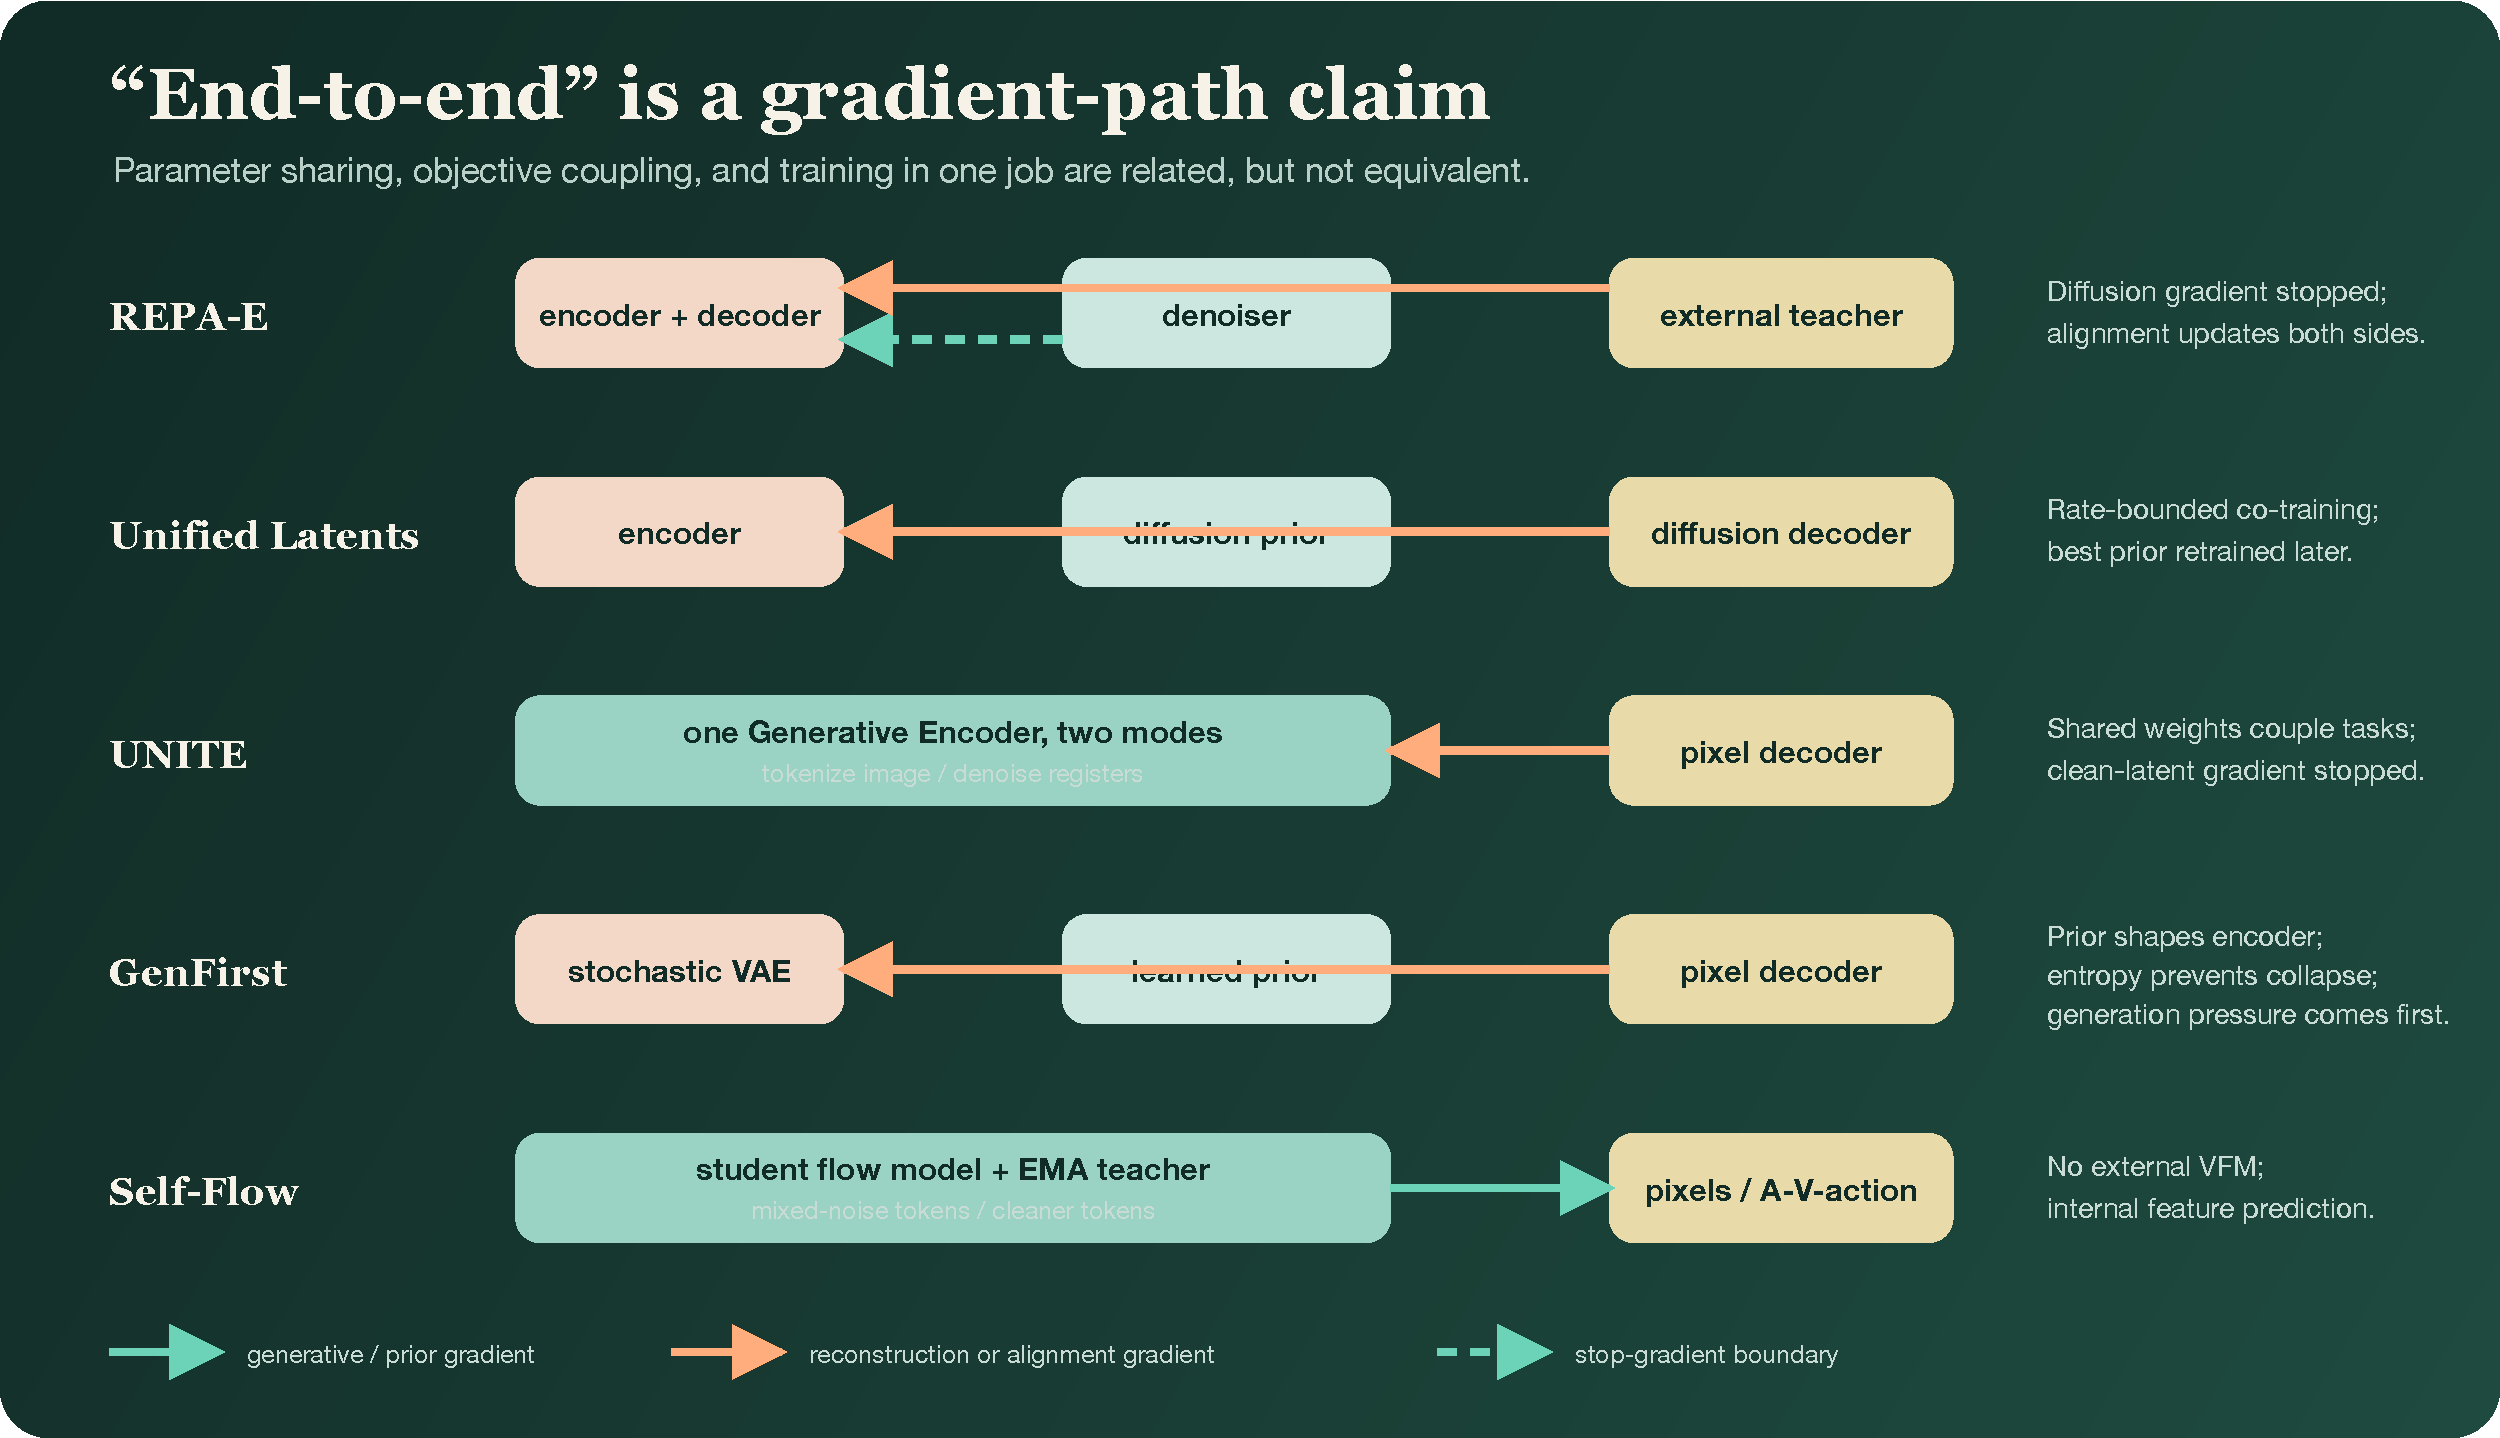
\includegraphics[width=\linewidth]{figures/gradient_paths_2026.pdf}
  \caption{Original comparison of dominant gradient paths. Similar forward pipelines can implement different optimization problems. A stop-gradient on the clean code does not imply complete independence when parameters are shared elsewhere.}
  \label{fig:gradients}
\end{figure}

\section{From Parallel Literatures to a Two-Axis Taxonomy}
\label{sec:history}

\subsection{Historical compression}

The VAE formalized amortized latent-variable learning \citep{kingma2014vae}; VQ-VAE supplied a learned discrete tokenizer \citep{oord2017vqvae}. Score-based latent models showed that a learned diffusion prior could be integrated with a hierarchical autoencoder \citep{vahdat2021lsgm}. Latent diffusion then established the modular engineering recipe: train a perceptual compressor, freeze it, and learn a denoiser in the compressed space \citep{rombach2022ldm}. DiT made the latent denoiser a scalable Transformer \citep{peebles2023dit}.

In parallel, self-supervised visual encoders developed increasingly transferable semantic spaces. Their features were usually evaluated by linear probes, retrieval, segmentation, or robustness, not by whether pixels could be reconstructed or whether a generative prior could model their full joint distribution. The convergence began when generative models used those features as internal targets. \method{REPA} aligned DiT hidden states to frozen semantic features and reported substantially faster optimization \citep{yu2024repa}. Follow-up work varied targets, schedules, and coupling, while another branch moved the alignment into the tokenizer. A third branch replaced the conventional VAE encoder with a VFM. The 2026 wave made the final step explicit: allow representation, prior, and decoder to shape one another.

\subsection{The taxonomy}

Figure~\ref{fig:taxonomy} separates two questions.

\paragraph{Where does the representation enter?}
(i) as an auxiliary target inside a denoiser; (ii) as a constraint on a tokenizer or VAE; (iii) as the generative latent itself; or (iv) inside a native pixel/data-space or multimodal model. These positions imply different inference costs and different failure modes.

\paragraph{How strongly is training coupled?}
A representation can be frozen, selectively adapted or staged, or jointly learned. Parameter sharing, gradient sharing, and schedule coupling are distinct. A frozen teacher can still strongly shape early optimization; a shared encoder can receive stopped clean-code gradients; a joint first stage can still be followed by a freshly trained prior.

\begin{figure*}[t]
  \centering
  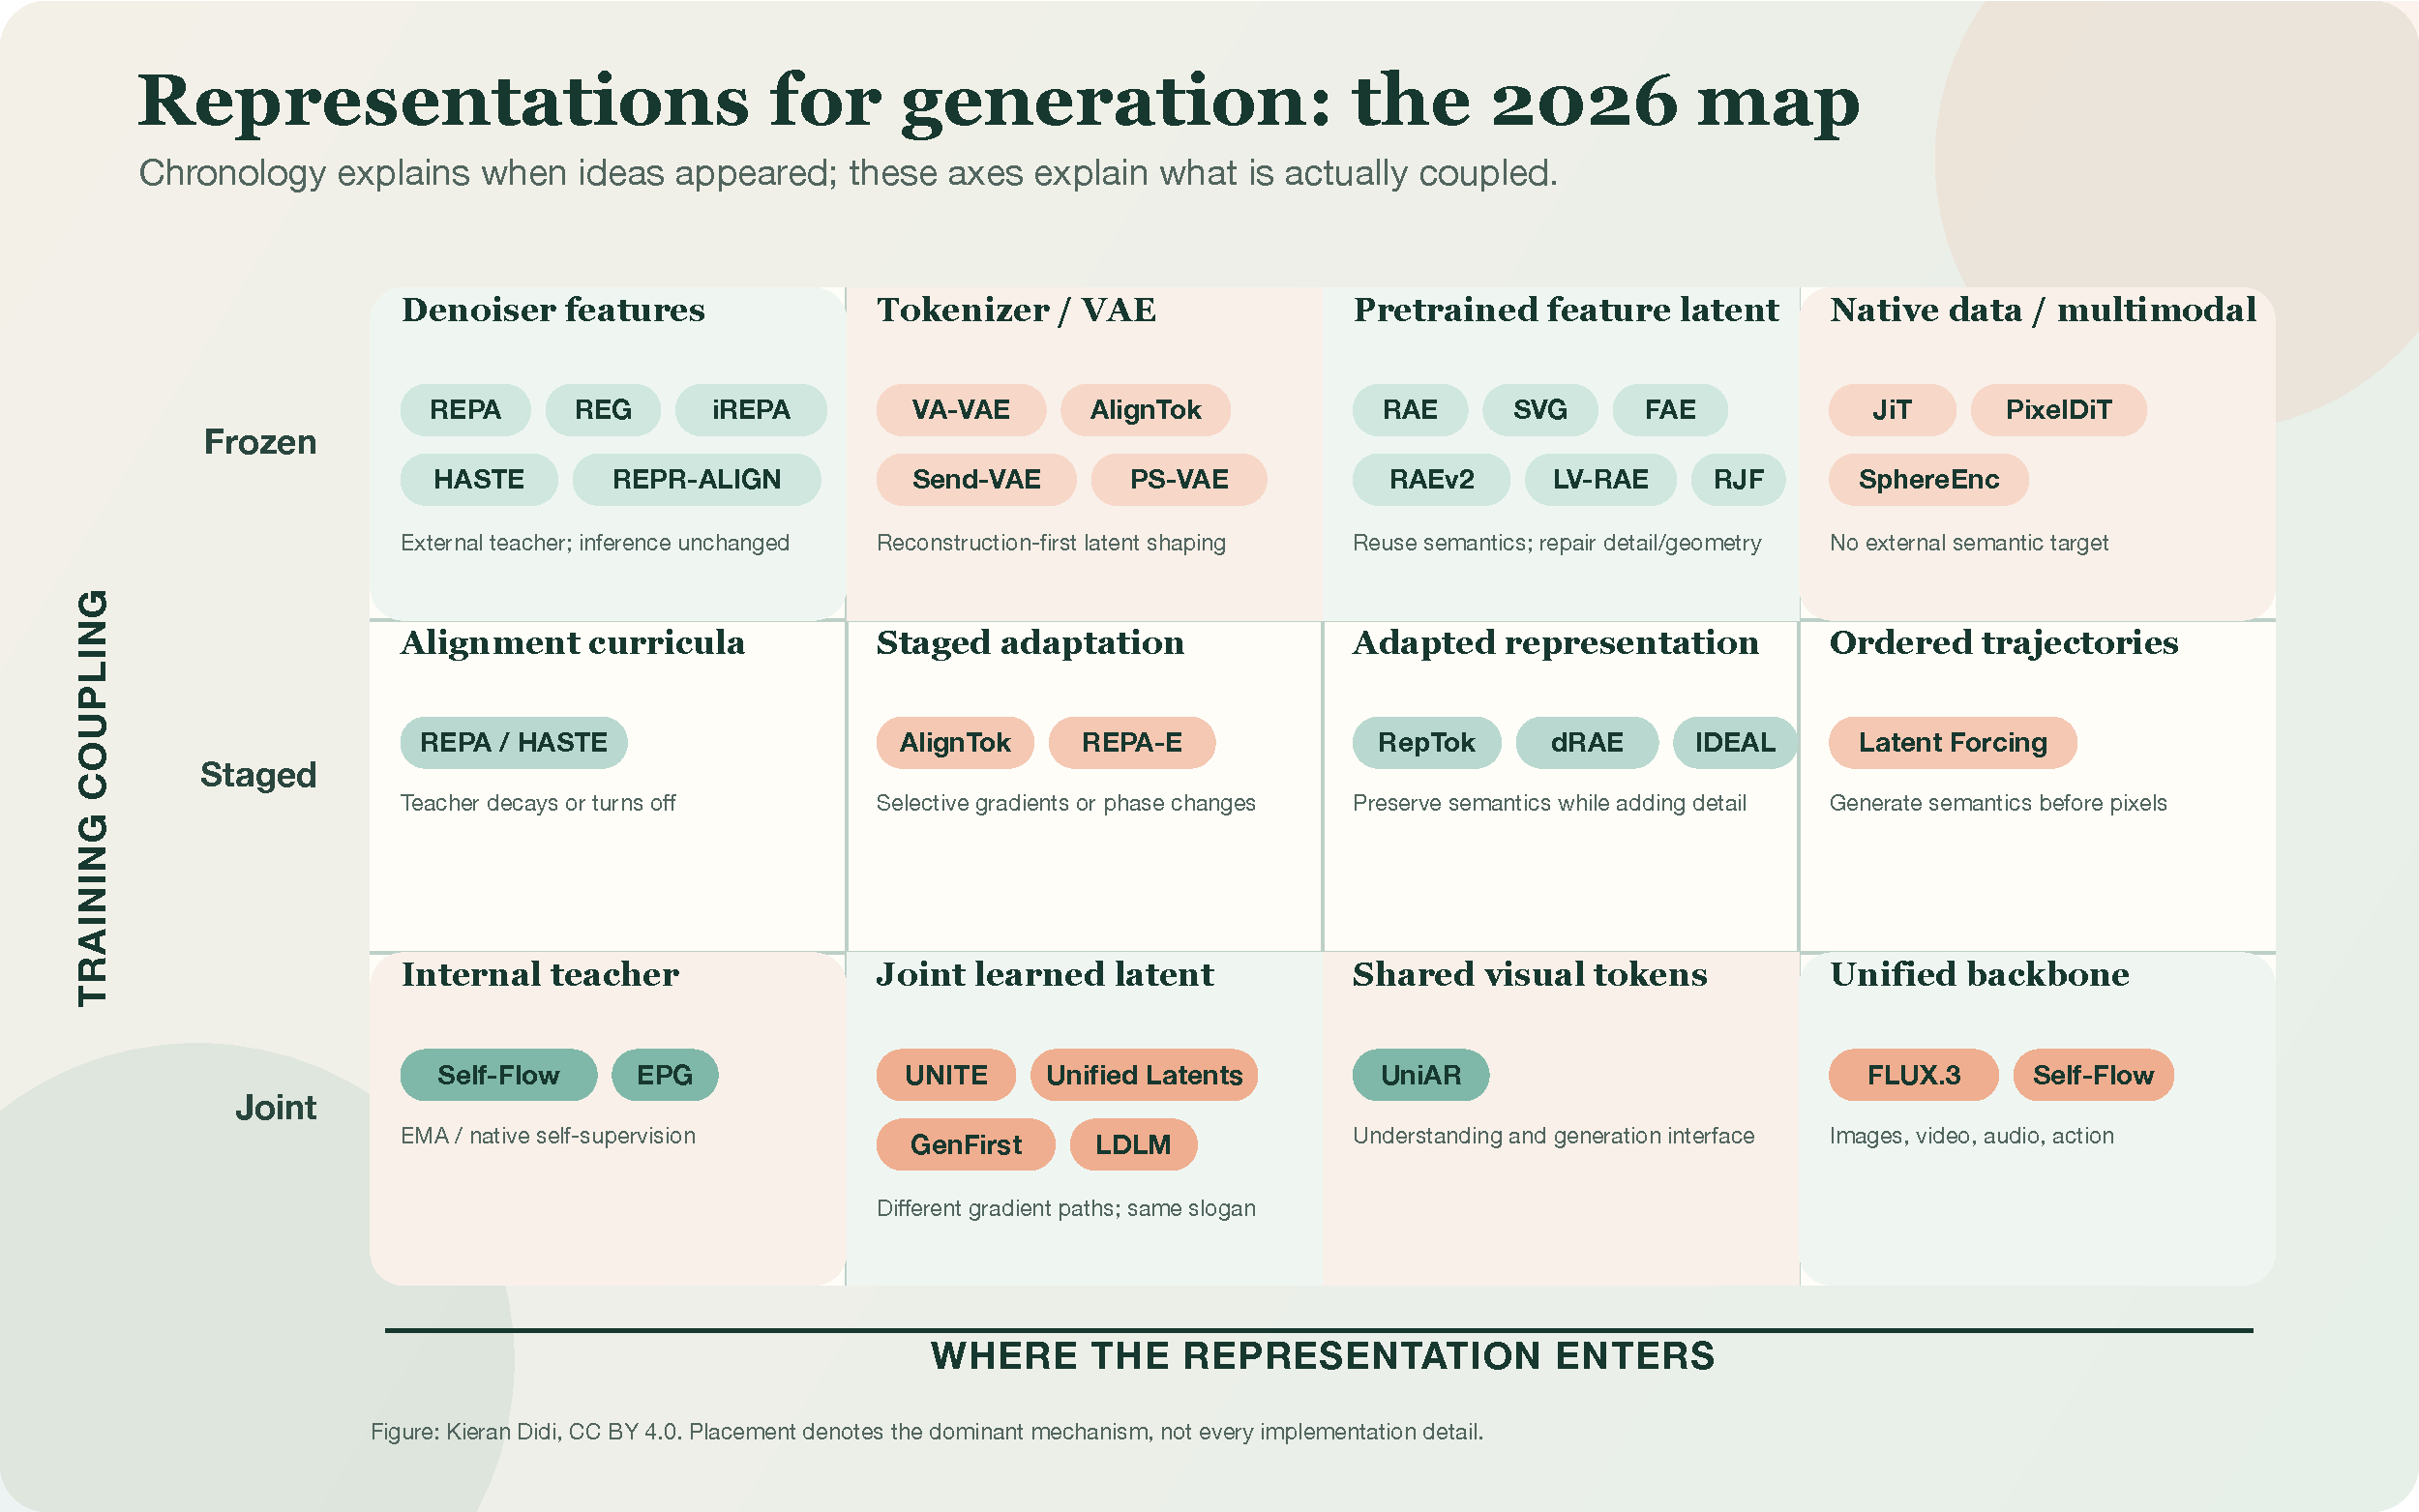
\includegraphics[width=0.96\textwidth]{figures/taxonomy_2026.pdf}
  \caption{A two-axis map of representative methods. Placement denotes the dominant mechanism rather than every implementation detail. Chronology explains when ideas appeared; these axes explain what is coupled. Original figure, CC BY 4.0.}
  \label{fig:taxonomy}
\end{figure*}

\begin{table*}[t]
\centering
\small
\setlength{\tabcolsep}{4.5pt}
\begin{tabularx}{\textwidth}{@{}p{2.2cm}p{2.35cm}p{2.15cm}p{2.25cm}X@{}}
\toprule
Family & Representation enters as & Typical coupling & Inference consequence & Diagnostic question \\
\midrule
Denoiser alignment & auxiliary hidden-state target & frozen teacher; scheduled weight & usually none & Does alignment accelerate useful features or overconstrain them? \\
Aligned tokenizer & regularizer or target for encoder & frozen teacher; encoder adapted & same latent pipeline & Which semantic invariances can reconstruction tolerate? \\
Representation AE & pretrained feature is the code & frozen/lightly adapted encoder & decoder must invert VFM space & Are semantic codes complete, normalized, and locally decodable? \\
Joint latent learning & learned interface among encoder, prior, decoder & shared or routed gradients & architecture dependent & Can prior pressure improve modelability without collapse? \\
Native/self-supervised & target generated by model or trajectory & joint/EMA & may remove external teacher & What asymmetry prevents a trivial target? \\
\bottomrule
\end{tabularx}
\caption{Mechanism-first comparison. The final column is more portable than any method label.}
\label{tab:families}
\end{table*}

\section{Auxiliary Representations Inside the Generator}
\label{sec:alignment}

\method{REPA} adds a semantic prediction task to intermediate denoiser features while leaving the VAE and inference graph unchanged \citep{yu2024repa}. This is attractive because the auxiliary loss is removable: one can improve optimization without paying for the teacher at sampling time. It also creates a clean experimental question about what feature target helps.

The answer is not simply the strongest recognition model. \method{What Matters for Representation Alignment} finds that spatial self-similarity is highly predictive in its controlled comparison, while global semantic quality alone is insufficient \citep{singh2025whatmatters}. The result is specific to using a representation as a patchwise denoiser target. It does not imply that global semantics are unimportant when the representation is the latent itself. Indeed, \method{RAEv2} reports benefits from globally semantic encoders while an added REPA-style objective improves spatial organization \citep{singh2026raev2}. The location of the representation changes the desired property.

Permanent alignment can also become a liability. \method{HASTE} reports that turning alignment off early preserves its optimization benefit while avoiding late-stage conflict \citep{wang2025haste}. \method{REG} entangles representation guidance more deeply with generative features \citep{wu2025reg}. These variants suggest three interpretations of Equation~\eqref{eq:repa}: representation alignment can be (i) a semantic regularizer, (ii) a preconditioner or curriculum that shapes early features, or (iii) an internal guidance signal. Experiments should distinguish them by sweeping the active interval, target layer, spatial granularity, and teacher.

\paragraph{Practical recipe.}
Normalize target and predicted features, isolate the alignment head from the output head, and report whether the teacher operates on clean images, decoded latents, or augmented views. Log the cosine loss by diffusion time. If alignment helps only at high noise or only early in training, a scheduled objective is more faithful than an always-on penalty. Evaluate generation after removing the head to verify that the claimed gain is carried by the denoiser rather than by an inference-time crutch.

\section{Shaping the Tokenizer and Adopting Pretrained Features}
\label{sec:tokenizers}

\subsection{Semantically aligned autoencoders}

Conventional perceptual autoencoders already borrow representation losses through LPIPS-like feature distances, but recent methods place semantic organization at the center. \method{REPA-E} allows a representation objective to update the VAE encoder while stopping the diffusion loss from flowing into that encoder \citep{leng2025repae}. Thus it is end-to-end in scheduling and system assembly, not in the strongest gradient-sharing sense. \method{AlignTok} adapts a VFM toward a compact tokenizer while trying to preserve useful semantic structure \citep{chen2025aligntok}. \method{PS-VAE} argues that both semantics and reconstruction are needed for text-to-image generation and editing \citep{zhang2025psvae}. Work on autoencoder diffusability likewise shows that reconstruction FID can improve while the latent distribution becomes harder to model \citep{skorokhodov2025diffusability}.

The optimization conflict is easy to state. Suppose a nuisance variable \(n\) affects pixels but not category. A representation objective may reward
\[
\enc{I(z;y)\ \text{large}},\qquad \enc{I(z;n)\ \text{small}},
\]
whereas an invertible decoder needs enough information about \(n\) to reconstruct \(x\). A practical tokenizer can allocate low-frequency or semantic information to an aligned subspace and residual detail to another, but this is an architectural compromise rather than a proof that semantics and fidelity are naturally identical.

\subsection{Representation autoencoders}

A representation autoencoder (RAE) uses a pretrained encoder \(E_{\mathrm{VFM}}\) as the image code and trains a decoder \(D_\psi\) to reconstruct pixels. The prior learns
\[
z_0=E_{\mathrm{VFM}}(x),\qquad
\mathcal{L}_{\mathrm{prior}}=\E\|v_\theta(z_t,t)-u_t\|^2.
\]
The promise is compelling: replace a low-level VAE code with a semantically organized representation and inherit the scaling of foundation-model pretraining. The cost is that the code may be high-dimensional, anisotropic, lossy in local detail, or concentrated near a curved manifold. A decoder trained only on exact encoder outputs may also be brittle to the approximate samples produced by the prior.

The original RAE work couples a frozen pretrained encoder with a learned pixel decoder and adapts the generative architecture to the resulting wide latent \citep{zheng2025rae}. Scaling studies show that conclusions depend on DiT width and encoder dimension \citep{tong2026scalerae}. \method{RAEv2} aggregates several encoder layers, compares 27 encoders, and combines the latent with internal representation guidance; its main lesson is that RAE and REPA are complementary, not mutually exclusive \citep{singh2026raev2}. \method{LV-RAE} restores low-level information and explicitly trains decoder robustness around the feature manifold \citep{liu2026lvrae}.

\method{FAE} is a useful boundary case. It keeps the VFM frozen but compresses its patch features using one self-attention layer plus a projection. A six-layer feature decoder reconstructs the original VFM feature field using feature MSE and a small KL term; a separate pixel decoder is trained on noisy original features and then refined on reconstructed features \citep{gao2026fae}. Only after this staged adaptation is a generative prior learned. It is therefore neither one projection and done nor a fully joint generator. Its claim is that a very small trainable bottleneck can preserve useful VFM geometry while restoring a conventional, compact generative interface.

\paragraph{Discrete and spherical variants.}
\method{IDEAL} aligns discrete codes with shallow and deep VFM features \citep{chen2026ideal}; \method{dRAE} uses hyperspherical codes to reduce sensitivity to feature magnitude \citep{ma2026drae}. \method{RAE-AR} addresses sequential generation by normalizing codes and injecting Gaussian noise during autoregressive training \citep{yu2026raear}. Here exposure bias has its sequence-model meaning: training sees ground-truth previous codes, whereas generation conditions on its own imperfect samples. This differs from poor reconstruction on clean features and from geometric path mismatch, even though all three can produce off-manifold decoder inputs.

\section{Jointly Learning the Latent Interface}
\label{sec:joint}

\subsection{Unified Latents: rate as a design variable}

\method{Unified Latents} uses a deterministic encoder followed by fixed Gaussian noise, a diffusion prior whose minimum noise matches the encoder noise, and a diffusion decoder \citep{heek2026ul}. The prior is trained with an unweighted diffusion ELBO, while reweighting the decoder ELBO controls which information remains in the latent. This construction makes rate explicit rather than treating latent dimension as its proxy.

For any auxiliary code distribution \(q_\phi(z\mid x)\) and prior \(p_\theta(z)\),
\begin{align}
\E_{p(x)}\KL(q_\phi(z\mid x)\|p_\theta(z))
&=
\underbrace{I_q(X;Z)}_{\enc{\text{information rate}}}
+
\underbrace{\KL(q_\phi(z)\|p_\theta(z))}_{\prior{\text{aggregate mismatch}}},
\label{eq:rate}
\end{align}
where \(q_\phi(z)=\int p(x)q_\phi(z\mid x)\,dx\). The expected prior cost upper-bounds mutual information because the second term is non-negative. It simultaneously charges for information in each code and for a prior that fails to match the aggregate posterior. UL operationalizes this relation with diffusion-based likelihood terms.

The nuance matters: encoder, prior, and decoder are co-trained in the first stage, but UL's strongest reported generation configuration freezes the learned autoencoder and trains a fresh prior afterward. This is evidence that joint training can learn a useful interface, not evidence that a single training job is always optimal.

\subsection{UNITE: shared weights with routed gradients}

\method{UNITE} uses one Generative Encoder in two modes: tokenization of clean data and denoising of corrupted latent tokens \citep{duggal2026unite}. Register tokens create a compact code, and the same core weights participate in representation formation and latent denoising. Yet the best configuration stops the denoising gradient at the clean latent. That stop-gradient does not make the tasks independent: the denoising mode still updates shared parameters, which subsequently changes tokenization. The coupling is \emph{through shared weights across modes}, not through direct differentiation of the prior loss through the clean-code computation.

This distinction explains why two statements can both be true: UNITE is an end-to-end shared model, and naive direct latent gradients can be harmful. The architecture couples the tasks while the stop-gradient controls a high-variance or collapse-prone route. UNITE also reports experiments on images, QM9 molecules, and MP20 crystals, making it unusually relevant to cross-domain transfer.

\subsection{GenFirst: give the prior a gradient, then prevent collapse}

\method{GenFirst} explicitly allows the generative prior to shape the encoder \citep{zheng2026genfirst}. Its diagnosis is that naive joint likelihood training contains pressure to reduce the entropy of the aggregate code because a concentrated distribution is easier for the prior. A schematic objective is
\begin{equation}
\mathcal{J}
=
\underbrace{\lambda_{\mathrm{rec}}\mathcal{L}_{\mathrm{rec}}}_{\dec{\text{retain information}}}
+
\underbrace{\lambda_{\mathrm{fit}}\mathcal{L}_{\mathrm{prior}}}_{\prior{\text{fit aggregate codes}}}
-
\underbrace{\lambda_H H(q_\phi(z))}_{\enc{\text{oppose collapse}}},
\label{eq:genfirst}
\end{equation}
combined with a generation-first schedule: prioritize a modelable latent before tightening reconstruction. The entropy term is not decorative. Without a countervailing force, the prior objective can be improved by mapping diverse \(x\) to similar \(z\).

GenFirst and UL therefore share the ambition to make rate and generation pressure part of representation learning, but their mechanisms differ. UL derives a variational rate-control construction with fixed encoder noise; GenFirst foregrounds entropy balance and curriculum. GenFirst, too, evaluates a freshly trained prior after learning the autoencoder, so end-to-end latent discovery and final prior training should be reported separately.

\begin{table*}[t]
\centering
\small
\setlength{\tabcolsep}{4pt}
\begin{tabularx}{\textwidth}{@{}p{1.45cm}p{2.3cm}p{2.15cm}p{2.1cm}p{2.15cm}X@{}}
\toprule
Method & Representation source & Prior gradient to clean encoder & Anti-collapse / control & Final prior protocol & Most precise description \\
\midrule
REPA-E & VAE encoder aligned to frozen VFM & \no & alignment and reconstruction & jointly scheduled DiT & encoder adaptation with routed gradients \\
UL & learned noisy continuous code & \yes & fixed noise and variational rate & strongest result retrains prior & joint interface learning with explicit rate \\
UNITE & shared Generative Encoder/registers & \no\ (best setting) & stop-gradient and mode sharing & shared latent denoiser & shared parameters, selectively routed gradient \\
GenFirst & learned continuous code & \yes & entropy term and curriculum & fresh prior also evaluated & prior-shaped representation with collapse control \\
\bottomrule
\end{tabularx}
\caption{Why end-to-end is not a sufficient method description.}
\label{tab:joint}
\end{table*}

\section{What Makes a Representation Generative?}
\label{sec:criteria}

We propose reporting six partly independent properties.

\paragraph{1. Reconstruction fidelity.}
Measure distortion in pixels and perceptual features, but also editing consistency and fine-structure recovery. Clean reconstruction tests \(D(E(x))\), not \(D(\tilde z)\) for prior samples \(\tilde z\).

\paragraph{2. Semantic organization.}
Linear probes, retrieval, segmentation, and robustness reveal whether downstream factors are accessible. They do not establish invertibility. Moreover, spatial and global semantics play different roles: patchwise denoiser alignment rewards spatial correspondence, while a latent prior may benefit from globally meaningful organization.

\paragraph{3. Information rate.}
Latent dimension alone is not rate. A continuous \(64\times64\times1024\) tensor can carry little information if heavily noised, or enormous information at high precision. Report an entropy or coding proxy, encoder noise, quantization, and the prior cross-entropy where possible. Equation~\eqref{eq:rate} provides a principled decomposition.

\paragraph{4. Distributional modelability.}
Whitening, channel scale, token outliers, covariance condition number, and tail behavior affect optimization. A generator can fail on a perfectly reconstructive latent simply because the aggregate distribution is ill-conditioned. Conversely, a low-dimensional smooth code may be easy to model while discarding details the decoder cannot recover.

\paragraph{5. Geometry and spectrum.}
If features concentrate on a sphere or another manifold, Euclidean interpolation can traverse low-density interiors. Hyperspherical methods such as \method{Sphere Encoder} and \method{dRAE} make the geometry explicit \citep{yue2026sphere,ma2026drae}. Frequency organization is another view. \method{Spectrum Matching} proposes that a diffusion-friendly encoder should expose a suitably flattened power spectrum and that decoder training should pair image- and latent-frequency perturbations \citep{ning2026spectrum}.

The exact foundation is Parseval's identity. For an orthonormal transform \(F\),
\begin{align}
\|x-\hat x\|_2^2
&=\|F(x-\hat x)\|_2^2 \nonumber\\
&=\sum_k
\underbrace{|(Fx)_k-(F\hat x)_k|^2}_{\prior{\text{error at frequency }k}}.
\label{eq:parseval}
\end{align}
Thus pixel MSE decomposes exactly by frequency. It does \emph{not} follow as a theorem that a particular flattened spectrum is sufficient or optimal for diffusion. The stronger spectrum-matching hypothesis is an empirically supported design hypothesis. It is complementary to rate and manifold geometry, not a replacement for them.

\paragraph{6. Decoder robustness.}
At inference, the decoder sees samples from the learned prior, not exact encoder outputs. Let \(\delta=\tilde z-E(x)\). Locally,
\[
D(E(x)+\delta)\approx D(E(x))+J_D(E(x))\delta.
\]
Even small latent error becomes large pixel error when the decoder Jacobian has high gain along likely prior-error directions. Noise injection, drifted-latent training, consistency losses, and explicit Jacobian control all target this mismatch. The right perturbation distribution should resemble actual prior errors rather than isotropic noise by default.

\begin{table*}[t]
\centering
\small
\begin{tabularx}{\textwidth}{@{}p{2.15cm}p{3.0cm}p{3.0cm}X@{}}
\toprule
Property & Useful measurements & Common proxy failure & Representative interventions \\
\midrule
Fidelity & PSNR/SSIM, rFID, LPIPS, edit recovery & clean recon ignores sampled latents & residual detail paths, richer decoder \\
Semantics & probes, retrieval, dense tasks & global probe hides spatial mismatch & REPA, multi-layer VFM features \\
Rate & nats/bits, prior NLL, encoder noise & tensor size is not information & UL weighting/noise, quantization \\
Modelability & prior loss, covariance, tails, convergence & rFID can improve while gFID worsens & normalization, compact bottleneck \\
Geometry /\newline spectrum & norm/radius, geodesic tests, PSD & Euclidean metrics ignore support & spherical codes, spectrum matching \\
Robustness & drifted-latent recon, Jacobian gain & \(D(E(x))\) is in-distribution only & noisy-feature or sampled-code training \\
\bottomrule
\end{tabularx}
\caption{A minimum diagnostic panel for generative representations.}
\label{tab:criteria}
\end{table*}

\section{Native and Self-Supervised Generative Representations}
\label{sec:native}

\subsection{Sphere Encoder and iterative refinement}

\method{Sphere Encoder} learns a conditionally uniform hyperspherical latent and samples directly from the sphere \citep{yue2026sphere}. It can generate in one decoder pass or refine by repeatedly encoding and decoding. This is not an RAE: the code is not inherited from a pretrained semantic encoder. It is also not a diffusion prior: the intent is to make a simple uniform prior directly usable. Its recurrence is best seen as learned projection or refinement around an autoencoder.

\subsection{Latent Forcing: order the information reveal}

\method{Latent Forcing} keeps pixel-space generation but jointly diffuses pixels and pretrained semantic features with separate time schedules \citep{baade2026latentforcing}. Denote noisy pixels \(x_{t_x}\) and noisy semantic features \(r_{t_r}\). A joint network predicts both flows:
\[
\mathcal{L}
=
\E\!\left[
\|v_x(x_{t_x},r_{t_r},t_x,t_r)-u_x\|^2
+
\lambda_r\|v_r(x_{t_x},r_{t_r},t_x,t_r)-u_r\|^2
\right].
\]
By choosing \(t_r\) to resolve semantics before \(t_x\) resolves pixels, the trajectory exposes a coarse semantic plan before high-frequency synthesis. This is trajectory design, not tokenizer learning. The paper's strongest schedule should not be generalized into a universal rule without considering modality and architecture.

\subsection{Self-Flow: the teacher is generated internally}

\method{Self-Flow} removes the external semantic teacher by creating asymmetric views of the same noisy sample \citep{chefer2026selfflow}. Tokens receive heterogeneous noise times. An exponential-moving-average (EMA) teacher observes a cleaner version, while the student observes mixed noise and predicts teacher features in addition to the flow target. Schematically,
\begin{align}
h^- &= f_{\bar\theta}(x_{\min(t,s)},\min(t,s)),\\
\mathcal{L}_{\mathrm{SF}}
&=
\underbrace{\|v_\theta(x_t,t)-u_t\|^2}_{\prior{\text{flow}}}
+
\lambda
\underbrace{\left[1-\cos(g(h_\theta(x_t,t,s)),\stopgrad(h^-))\right]}_{\teacher{\text{internal feature target}}}.
\label{eq:selfflow}
\end{align}
The EMA, stop-gradient, and cleaner-context asymmetry prevent the target from trivially chasing the student. The method spans image, video, audio, multimodal, and action experiments, with modality-specific schedules. It removes dependence on an external VFM; it does not imply the absence of an autoencoder or tokenizer in every implementation.

\paragraph{Product-scale evidence.}
Black Forest Labs states that \method{FLUX.3} builds on Self-Flow and uses a shared flow-matching backbone across image, video, audio, and action generation \citep{bfl2026flux3}. This is relevant evidence that the design family is being scaled, but the public report describes evaluations as preliminary and does not disclose enough detail for independent reproduction. It should be cited as a first-party system announcement, not counted as a controlled research comparison.

\section{Beyond Images}
\label{sec:beyond}

\subsection{Language and unified multimodal models}

\method{LDLM} jointly adapts pretrained language features, a latent diffusion model, and a decoder \citep{meshchaninov2026ldlm}. It uses a hidden-state reconstruction loss, a warm-up that delays difficult coupling, adaptive timestep sampling, and noise on decoder inputs. These stabilizers mirror the visual literature: control the gradient path, teach the decoder about inference-time drift, and allocate optimization effort where the prior is weakest.

\method{REPR-ALIGN} takes the opposite direction, adapting an autoregressive language model toward diffusion through representation alignment rather than fully retraining it \citep{peng2026repralign}. \method{UniAR} argues that a shared context-visual tokenizer is central to unified autoregressive understanding and generation \citep{peng2026uniar}. Controlled 2026 studies report that generation and understanding can transfer when they require shared knowledge, but also identify asymmetric interference when both are forced through identical computation paths \citep{zhu2026vgaudiag,wu2026synergy}. Unified should therefore be decomposed into shared vocabulary, shared latent, shared trunk, shared objective, and shared inference procedure.

\subsection{Molecules, proteins, and 3D scenes}

Structural domains sharpen the interface problem because validity is geometric. Rotations and translations should not change identity; atom order may be arbitrary; chirality matters; structures vary in size; and a small local coordinate error can propagate globally. A semantic image feature can discard texture harmlessly, whereas a protein code that discards stereochemistry is chemically wrong.

\method{UNITE} reports the same shared tokenization/denoising mechanism on QM9 molecules and MP20 crystals as well as images \citep{duggal2026unite}. \method{Kanzi} uses a flow-matching decoder as a compact protein-structure tokenizer and reports strong reconstruction with a much smaller model than specialized geometric tokenizers \citep{dilip2026kanzi}. \method{OneWorld} builds a 3D unified representation autoencoder from pretrained 3D features, adds cross-view consistency, and trains on both clean and drifted representations \citep{gao2026oneworld}. These examples support the transfer of \emph{principles}---rate, geometry, and decoder robustness---not the literal reuse of image architectures.

Protein modeling also clarifies the difference between representation recurrence and generative self-conditioning. AlphaFold recycling repeatedly feeds predicted structure-derived features back through the network to refine one prediction \citep{jumper2021alphafold}; ESMFold uses a related folding trunk around language-model features \citep{lin2023esmfold}. RFdiffusion uses diffusion self-conditioning in structure generation \citep{watson2023rfdiffusion}. The generic diffusion technique predates RFdiffusion: Analog Bits explicitly introduced self-conditioning of a model's previous clean-data estimate for discrete diffusion \citep{chen2023selfcondition}. Recycling, self-conditioning, and iterative decoding all feed predictions forward, but differ in state, objective, and stochastic semantics. Appendix~\ref{app:recurrence} makes the distinction precise.

\section{Evaluation and Reporting}
\label{sec:evaluation}

\subsection{Why headline FID is insufficient}

Generation FID depends on training data, resolution, sample count, guidance scale, number of function evaluations, sampler, model size, augmentation, and evaluation implementation. Reconstruction FID depends on the decoder and on whether stochasticity is used. Reporting a lower number across papers does not identify which representation is better unless these variables are controlled.

At minimum, a representation paper should report:
\begin{enumerate}[leftmargin=*]
  \item clean reconstruction and reconstruction under realistic latent drift;
  \item unconditional or class/text-conditional generation with and without guidance;
  \item latent rate or a defensible proxy, spatial size, channel count, normalization, and encoder noise;
  \item prior convergence curves at matched compute, not only the best checkpoint;
  \item semantic and dense/spatial probes where relevant;
  \item all stop-gradients, frozen modules, EMA targets, warm-ups, and stage boundaries; and
  \item final-prior protocol, especially whether a new prior is trained after joint latent learning.
\end{enumerate}

\subsection{Ablations that answer causal questions}

An informative ablation changes one interface property while holding capacity and compute fixed. Examples include whitening versus raw features; identical decoder with clean versus drifted-latent training; equal-rate latents with different dimensions; direct prior-to-encoder gradient versus stop-gradient under the same shared trunk; and aligned targets with preserved versus shuffled spatial structure. Scaling only the denoiser may hide a difficult latent rather than repair it.

The most useful negative results are boundary conditions. If representation alignment stops helping after early training, that locates its role as curriculum. If a VFM latent helps a wide DiT but not a narrow one, architecture and representation are coupled. If fresh-prior retraining improves a jointly learned system, that distinguishes interface discovery from final density estimation. Such findings are more reusable than a single champion configuration.

\section{Synthesis: What the 2026 Wave Changes}
\label{sec:synthesis}

The 2026 papers do not replace the earlier story; they split several overloaded concepts.

\paragraph{End-to-end is a family of gradient graphs.}
\method{REPA-E} aligns the encoder but blocks the diffusion gradient. \method{UNITE} shares weights across tokenization and denoising but performs best with a stopped clean code. UL co-trains encoder, prior, and decoder under a variational rate construction, then obtains its strongest generation with a fresh prior. GenFirst deliberately transmits prior pressure to the encoder and introduces entropy and curriculum to prevent collapse. These are not cosmetic variants.

\paragraph{Representation quality is multidimensional.}
\method{Spectrum Matching} adds frequency organization; spherical methods add explicit topology; UL adds rate; \method{LV-RAE} and OneWorld add decoder robustness; \method{RAE-AR} adds sequential exposure bias. No one diagnostic subsumes the others.

\paragraph{Internal teachers reduce dependence on external encoders.}
Self-Flow shows that heterogeneous-noise prediction and an EMA teacher can create useful targets within the generator. Latent Forcing shows that a pretrained semantic track can instead order the generation trajectory. Their shared lesson is controlled information asymmetry, not that all representations should be discarded.

\paragraph{Unification benefits from specialization with communication.}
Shared representations can transfer knowledge between understanding and generation, but fully identical paths can interfere. A common interface with mode-specific heads, schedules, or routed gradients may be more effective than one undifferentiated state.

\section{Limitations and Open Problems}

This survey reflects a rapidly moving literature and a September 2026 cutoff. Many works have not completed peer review; code availability and reported status may change. We emphasize primary papers and official project material, but cannot normalize every training and evaluation protocol. Our taxonomy assigns a dominant mechanism, which necessarily compresses hybrids.

Several research questions appear durable:
\begin{enumerate}[leftmargin=*]
  \item Can latent rate, prior difficulty, and decoder robustness be measured in a common evaluation rather than inferred from architecture?
  \item Which prior-error distribution should a decoder train against, and can it be estimated online without destabilizing joint learning?
  \item When does a curved manifold require a geometry-aware probability path rather than normalization or increased model width?
  \item Can a joint objective adapt semantic features while certifiably preserving downstream capabilities?
  \item What is the correct information ordering for video, audio, language, and 3D structures?
  \item How should unified systems allocate shared versus specialized capacity as modalities and tasks scale?
\end{enumerate}

\section{Conclusion}

The field is converging on a simple but demanding idea: a generative latent is an interface, not a by-product. Alignment methods change internal optimization; tokenizer methods decide which information is retained; RAEs inherit semantic geometry and its defects; joint methods let the prior reshape the code but must control collapse; native self-supervision creates targets from the generative process itself.

The practical rule is to inspect three objects together: the information carried by \(z\), the errors made by the prior, and the decoder's response to those errors. Then trace every gradient. This view explains why reconstruction, semantics, spectrum, geometry, and rate can each matter without any one becoming the universal answer. It also scales beyond images: the constraints change, but the interface-design problem remains.

\paragraph{Author's note.}
This article represents the author's personal scholarly synthesis and does not necessarily reflect the views of NVIDIA. Original text and figures are released under CC BY 4.0. No third-party paper figures are reproduced.

\bibliographystyle{plainnat}
\bibliography{references}

\appendix

\section{Detailed Derivations}
\label{app:derivations}

\subsection{The VAE bound, line by line}

Starting from the marginal likelihood and multiplying by one,
\begin{align}
\log p(x)
&= \log\int p(x,z)\,dz
&&\text{\color{softgray}{(marginalize \(z\))}}\\
&= \log\int q_\phi(z\mid x)\frac{p(x,z)}{q_\phi(z\mid x)}\,dz
&&\text{\color{softgray}{(importance identity)}}\\
&= \log \E_{q_\phi(z\mid x)}
\left[\frac{p_\psi(x\mid z)p(z)}{q_\phi(z\mid x)}\right]\\
&\ge \E_{q_\phi(z\mid x)}
\left[\log p_\psi(x\mid z)+\log p(z)-\log q_\phi(z\mid x)\right]
&&\text{\color{softgray}{(Jensen)}}\\
&=
\underbrace{\E_q[\log p_\psi(x\mid z)]}_{\dec{\text{decoder likelihood}}}
-
\underbrace{\KL(q_\phi(z\mid x)\|p(z))}_{\prior{\text{rate and regularity}}}.
\end{align}
The gap equals \(\KL(q_\phi(z\mid x)\|p(z\mid x))\), so the bound is tight when the approximate posterior matches the true posterior. Intuitively, the encoder sends a message \(z\); reconstruction rewards useful bits, while the KL charges for messages that are surprising under the prior.

\subsection{Why the expected prior cost contains mutual information}

Let \(q(x,z)=p_{\mathrm{data}}(x)q_\phi(z\mid x)\). Add and subtract \(\log q_\phi(z)\):
\begin{align}
\E_{p(x)}\KL(q(z\mid x)\|p(z))
&=\E_{q(x,z)}
\left[\log\frac{q(z\mid x)}{p(z)}\right]\\
&=\E_{q(x,z)}
\left[
\underbrace{\log\frac{q(z\mid x)}{q(z)}}_{\enc{\text{mutual information}}}
+
\underbrace{\log\frac{q(z)}{p(z)}}_{\prior{\text{aggregate mismatch}}}
\right]\\
&=I_q(X;Z)+\KL(q(z)\|p(z)).
\end{align}
The second term vanishes only when the prior exactly matches the aggregate posterior. A stronger learned prior can reduce aggregate mismatch without reducing the information rate. This is why latent dimension and prior loss should not be used interchangeably.

\subsection{Noise prediction, clean prediction, and velocity}

From \(z_t=\alpha_t z_0+\sigma_t\epsilon\), any two of \(z_t,z_0,\epsilon\) determine the third:
\[
\hat z_0=\frac{z_t-\sigma_t\hat\epsilon}{\alpha_t},
\qquad
\hat\epsilon=\frac{z_t-\alpha_t\hat z_0}{\sigma_t}.
\]
Define velocity \(v_t=\alpha_t\epsilon-\sigma_t z_0\). Then
\[
\begin{bmatrix}z_t\\v_t\end{bmatrix}
=
\begin{bmatrix}\alpha_t&\sigma_t\\-\sigma_t&\alpha_t\end{bmatrix}
\begin{bmatrix}z_0\\\epsilon\end{bmatrix},
\quad
\begin{bmatrix}z_0\\\epsilon\end{bmatrix}
=
\begin{bmatrix}\alpha_t&-\sigma_t\\\sigma_t&\alpha_t\end{bmatrix}
\begin{bmatrix}z_t\\v_t\end{bmatrix}.
\]
The matrix is orthogonal when \(\alpha_t^2+\sigma_t^2=1\). Thus the parameterizations encode equivalent targets at population optimum, but their finite-capacity weighting and numerical conditioning differ by timestep.

\subsection{Why naive prior pressure can collapse a learned code}

Consider a deterministic encoder \(z=E_\phi(x)\) and a flexible prior trained by negative log likelihood,
\[
\mathcal{L}_{\mathrm{prior}}=-\E_x\log p_\theta(E_\phi(x)).
\]
If the decoder term is weak, mapping every input to a constant \(z_\star\) makes the aggregate code maximally concentrated and easy for the prior to fit. A reconstruction loss resists because one code cannot reconstruct all inputs. An entropy reward resists directly:
\[
\mathcal{J}=
\dec{\lambda_{\mathrm{rec}}\mathcal{L}_{\mathrm{rec}}}
+
\prior{\lambda_{\mathrm{fit}}\mathcal{L}_{\mathrm{prior}}}
-
\enc{\lambda_H H(q_\phi(z))}.
\]
This toy argument does not prove a particular algorithm stable; it explains why letting the prior shape the encoder requires an opposing information-preservation mechanism.

\subsection{Spectrum matching and the limit of Parseval}

Let \(F\) be an orthonormal discrete Fourier or cosine transform, so \(F^\top F=I\). Then
\begin{align}
\|x-\hat x\|_2^2
&=(x-\hat x)^\top(x-\hat x)\\
&=(x-\hat x)^\top F^\top F(x-\hat x)
&&\text{\color{softgray}{(orthonormality)}}\\
&=\|F(x-\hat x)\|_2^2
=\sum_k |(Fx)_k-(F\hat x)_k|^2.
\end{align}
If a binary frequency mask \(M\) is applied consistently, the loss becomes
\[
\|M\odot F(x-\hat x)\|_2^2
=\sum_{k:M_k=1}|(Fx)_k-(F\hat x)_k|^2.
\]
This exactly justifies frequency-resolved reconstruction. It does not identify the optimal latent power spectral density. That step requires assumptions about the data, model class, noise schedule, and optimization, or empirical validation.

\subsection{Decoder robustness as a directional problem}

For prior sample error \(\delta\), first-order propagation gives
\[
\E\|D(z+\delta)-D(z)\|_2^2
\approx
\E\left[\delta^\top J_D(z)^\top J_D(z)\delta\right].
\]
If \(\Sigma_\delta=\E[\delta\delta^\top]\), then
\[
\E\|J_D\delta\|^2
=\operatorname{tr}\!\left(J_D^\top J_D\Sigma_\delta\right).
\]
Isotropic noise training uses \(\Sigma_\delta=\sigma^2I\) and penalizes average Jacobian energy. Actual prior errors can be anisotropic, concentrating along difficult directions. Sampling the current prior or fitting a local error covariance can therefore train the decoder more efficiently than indiscriminate isotropic perturbation.

\section{Self-Conditioning, Recycling, Looping, and Recurrence}
\label{app:recurrence}

These labels describe a shared computational motif---feed an intermediate prediction back into later computation---but not a shared probabilistic object.

\paragraph{Self-conditioning in diffusion.}
At step \(t\), a denoiser consumes a previous estimate of the clean sample,
\[
\hat x_0^{(t)}=f_\theta(x_t,t,\stopgrad(\hat x_0^{(t+1)})).
\]
Analog Bits used this technique for discrete-data diffusion before RFdiffusion adopted it for protein structures \citep{chen2023selfcondition,watson2023rfdiffusion}. The stop-gradient means the previous estimate acts as an auxiliary condition during ordinary training. It changes the parameterized reverse kernel while preserving a valid generative procedure if the augmented state and training/inference conditioning are defined consistently. What is usually lost is the simplicity of a Markov kernel written only as \(p_\theta(x_{t-1}\mid x_t)\): the implementation depends on cached model state. It does not automatically invalidate diffusion, but likelihood or ELBO statements derived for the unaugmented Markov chain cannot be quoted without modification.

\paragraph{Recycling.}
AlphaFold recycling maps a current structure and pair/single representations back into the folding trunk to refine the same prediction \citep{jumper2021alphafold}. It is supervised iterative inference, not a stochastic diffusion-time transition. Parameter sharing makes the unfolded computation recurrent. Training may unroll a limited number of recycles and stop gradients through earlier iterations for memory or stability.

\paragraph{Looping and generic recurrence.}
A looped Transformer reapplies a block \(h_{k+1}=F_\theta(h_k,x)\), often with shared weights. Backpropagation through time (BPTT) differentiates through the unrolled chain:
\[
\frac{\partial \mathcal{L}}{\partial\theta}
=\sum_{k=0}^{K-1}
\frac{\partial\mathcal{L}}{\partial h_K}
\left(\prod_{j=k+1}^{K-1}\frac{\partial h_{j+1}}{\partial h_j}\right)
\frac{\partial h_{k+1}}{\partial\theta}.
\]
The Jacobian product explains exploding or vanishing gradients and motivated gated recurrent networks \citep{hochreiter1997lstm}. Truncated BPTT stops some paths and optimizes a surrogate.

\paragraph{Deep equilibrium models.}
A deep equilibrium model defines \(h^\star=F_\theta(h^\star,x)\) and solves for the fixed point rather than storing all iterations \citep{bai2019deep}. Implicit differentiation gives
\[
\frac{dh^\star}{d\theta}
=
\left(I-\frac{\partial F_\theta}{\partial h}\bigg|_{h^\star}\right)^{-1}
\frac{\partial F_\theta}{\partial\theta}\bigg|_{h^\star}.
\]
DEQs are therefore a mathematically important ancestor of learned iterative refinement, but most recycling or self-conditioning systems are finite unrollings and do not enforce convergence to a fixed point. The useful connection is shared-weight computation and stability analysis; equality of names is not evidence of an equilibrium model.

\begin{table*}[t]
\centering
\small
\begin{tabularx}{\textwidth}{@{}p{2.2cm}p{2.5cm}p{2.1cm}p{2.1cm}X@{}}
\toprule
Mechanism & Feedback state & Index being iterated & Typical training gradient & Probabilistic role \\
\midrule
Diffusion self-conditioning & previous \(\hat x_0\) & noise/sampling time & often stopped through cached estimate & augments reverse-kernel context \\
Protein recycling & structure, single/pair features & refinement recycle & finite unroll or stopped earlier recycle & iterative supervised inference \\
Looped Transformer & hidden state or tokens & depth step & BPTT or truncation & architecture dependent \\
DEQ & equilibrium hidden state & root-solver iteration & implicit differentiation & implicit layer, not inherently generative \\
Sphere Encoder refinement & re-encoded decoded sample & refinement loop & method-specific finite loop & moves sample toward learned data manifold \\
\bottomrule
\end{tabularx}
\caption{Related computation patterns with different states, objectives, and theoretical commitments.}
\label{tab:recurrence}
\end{table*}

\section{Method Cards for the 2026 Additions}
\label{app:cards}

\paragraph{Unified Latents \citep{heek2026ul}.}
Intervention: learned continuous code. Coupling: joint encoder/prior/decoder first stage. Distinctive control: fixed encoder noise matched to the prior's minimum noise and a reweighted decoder ELBO. Caveat: strongest generation includes fresh-prior retraining.

\paragraph{UNITE \citep{duggal2026unite}.}
Intervention: one register-token Generative Encoder serves tokenizer and latent-denoising modes. Coupling: shared parameters, with stopped clean-code gradient in the best setting. Evidence: images plus QM9 and MP20. Caveat: shared weights should not be described as unrestricted gradient sharing.

\paragraph{GenFirst \citep{zheng2026genfirst}.}
Intervention: jointly learned latent shaped directly by the prior. Coupling: active prior-to-encoder gradient. Distinctive control: entropy counterterm and generation-before-reconstruction schedule. Caveat: code was pending at the survey cutoff, and a fresh final prior remains part of the evaluation.

\paragraph{FAE \citep{gao2026fae}.}
Intervention: compact bottleneck on frozen VFM features. Coupling: staged. Distinctive control: one-layer encoder, deeper feature decoder, and separate pixel decoder exposed to noisy features. Caveat: one layer describes the adapter, not the entire autoencoding system.

\paragraph{Spectrum Matching \citep{ning2026spectrum}.}
Intervention: encoder latent spectrum and decoder frequency training. Coupling: tokenizer-level. Distinctive control: encoding spectrum matching, decoding spectrum matching, and a Difference-of-Gaussians alignment target. Caveat: the algebraic decomposition is exact; the proposed preferred spectrum is empirical.

\paragraph{Sphere Encoder \citep{yue2026sphere}.}
Intervention: learned hyperspherical code with a simple uniform prior. Coupling: learned generative autoencoder. Distinctive control: conditional uniformity and optional iterative refinement. Caveat: neither a pretrained-feature RAE nor a diffusion prior.

\paragraph{Latent Forcing \citep{baade2026latentforcing}.}
Intervention: an auxiliary semantic trajectory in pixel diffusion. Coupling: joint dual-track denoising with separately scheduled times. Distinctive control: semantics resolve before pixels. Caveat: no learned tokenizer is implied.

\paragraph{Self-Flow and FLUX.3 \citep{chefer2026selfflow,bfl2026flux3}.}
Intervention: internal EMA representation target from a cleaner view. Coupling: native self-supervised flow training. Distinctive control: heterogeneous token timesteps and cross-time prediction. Caveat: the academic method has technical detail; FLUX.3 is a first-party deployment report with preliminary evaluation.

\section{Expanded Molecular and Structural Case Study}
\label{app:molecules}

The six-property framework changes meaning in structural domains:
\begin{description}[leftmargin=2.8cm,style=nextline,nosep]
\item[Fidelity] Bond lengths, local frames, clashes, chirality, and long-range topology matter; a perceptually plausible structure may still be chemically invalid.
\item[Semantics] Functional family, fold, secondary structure, or energy landscape can be more relevant than image-style class labels.
\item[Rate] Variable-size structures complicate per-sample comparisons. Report bits or nats per atom/residue as well as token count.
\item[Modelability] Equivariant coordinate distributions and discrete sequence/structure mixtures require different priors.
\item[Geometry] SE(3) symmetry, periodic boundary conditions, and manifold-valued rotations are first-class constraints rather than optional regularizers.
\item[Robustness] Small local-frame or torsion errors can accumulate along a chain; decoder training should reflect the error modes of the structure prior.
\end{description}

This makes the analogy to visual RAEs useful but incomplete. A pretrained 3D encoder can provide semantics, yet its invariances may remove precisely the degrees of freedom required for generation. Cross-view or equivariant consistency can preserve identity while avoiding arbitrary coordinate frames. Drifted-latent decoder training is especially important when validity depends on coordinated global constraints.

UNITE's cross-domain experiments suggest that shared register-token interfaces can survive a change in data type \citep{duggal2026unite}. Kanzi suggests that flow-based decoding itself can be an efficient tokenizer design \citep{dilip2026kanzi}. OneWorld demonstrates pretrained 3D features, cross-view consistency, and exposure to drifted representations \citep{gao2026oneworld}. The open question is not whether RAE for molecules works in the abstract, but which invariances, rates, and perturbations correspond to the downstream structural generator.

\section{Reading-Group Guide}
\label{app:reading}

A 60-minute discussion can be organized around five questions:
\begin{enumerate}[leftmargin=*]
  \item \textbf{10 min: What is the interface?} Derive Equations~\eqref{eq:elbo} and \eqref{eq:rate}; separate distortion, rate, and aggregate prior mismatch.
  \item \textbf{12 min: Where does representation enter?} Use Figure~\ref{fig:taxonomy} to contrast denoiser alignment, tokenizer shaping, RAEs, and native systems.
  \item \textbf{15 min: What does end-to-end mean?} Trace Figure~\ref{fig:gradients} and Table~\ref{tab:joint}; ask which gradient each stabilizer blocks.
  \item \textbf{13 min: What makes a latent modelable?} Debate whether rate, geometry, spectrum, or decoder robustness explains each result.
  \item \textbf{10 min: Does the analogy transfer?} Compare image latents with language and molecular structures, then identify broken invariances.
\end{enumerate}

\paragraph{Suggested core reading.}
Read REPA \citep{yu2024repa} for auxiliary alignment, RAE \citep{zheng2025rae} for pretrained-feature latents, and either UL \citep{heek2026ul} or GenFirst \citep{zheng2026genfirst} for joint latent learning. Add Spectrum Matching \citep{ning2026spectrum} for diagnostics and Self-Flow \citep{chefer2026selfflow} for native self-supervision. UNITE \citep{duggal2026unite} is the best bridge to non-image domains in this set.

\end{document}
